\documentclass[10pt,a4paper]{article}

\usepackage[utf8]{inputenc}
\usepackage[margin=1.2in]{geometry}
\usepackage[english]{babel}
\usepackage{amsmath}
\usepackage{amsfonts}
\usepackage{graphicx}
\usepackage{hyperref}
\usepackage[nottoc, notlof, notlot]{tocbibind}
\hypersetup{colorlinks=true,citecolor=black,filecolor=black,linkcolor=black,urlcolor=black}
\setlength{\parindent}{0.6cm} 
\setlength{\parskip}{0.10cm}
\usepackage[automark]{scrpage2}
\usepackage{color, colortbl}
\usepackage[table]{xcolor}
\usepackage{verbatim}
\usepackage{comment}


\pagestyle{scrheadings}

\ihead[]{TurtleTeam}
\ohead[]{Manuel Utilisateur - Navigation Autonome de Robot Mobile}


\begin{document}
\pagestyle {plain}

\begin{titlepage}


\newcommand{\HRule}{\rule{\linewidth}{0.5mm}} 

\center

\textsc{\Large Université Paul Sabatier Toulouse III}\\[1cm] 

\includegraphics[scale=0.3]{UPS.jpg}\\[0.6cm] 


\textsc{Master 2 Intelligence Artificielle et \\ 
Reconnaissance des Formes \\ Master 2 Robotique : Décision et Commande}\\[3cm] 

\HRule \\[0.4cm]
{ \huge \bfseries Navigation Autonome de Robot Mobile}\\[0.4cm] 
\LARGE Manuel Utilisateur

\HRule \\[1.5cm]
 

\begin{minipage}{0.4\textwidth}
\begin{flushleft} \large
\emph{Auteurs:}\\
\href{mailto:beauhaire.pierre@gmail.com}{Pierre \textsc{Beauhaire} }  \\
\href{mailto:brefel.hugo@gmail.com}{Hugo \textsc{Brefel} }  \\
\href{mailto:salaheddineghamri@gmail.com}{Salah Eddine \textsc{Ghamri} } \\
\href{mailto:sylvain31g@free.fr}{Sylvain \textsc{Guillaume} } \\
\href{mailto:luc.rubio.lr@gmail.com}{Luc \textsc{Rubio} } 
\end{flushleft}
\end{minipage}
~
\begin{minipage}{0.4\textwidth}
\begin{flushright} \large
\emph{Tuteurs:} \\
\href{mailto:michael.lauer@laas.fr}{Michaël \textsc{LAUER}} \\
\href{mailto:lerasle@laas.fr}{Frédéric \textsc{LERASLE}}\\
\href{mailto:taix@laas.f}{Michel \textsc{TAIX}}
\end{flushright}
\end{minipage}\\[5cm]


\large Mars 2018
 

\end{titlepage}

\newpage


\subsection*{Suivi du document}

\begin{center}
    \begin{tabular}{| l | l | l | l | l |}
    \hline
     \rowcolor{gray} Nom & Version & Date de création \\ \hline
    Manuel Utilisateur - & 1 & 21/03/2017 \\ 
    Navigation autonome & & \\ 
    de Robot Mobile &  & \\ \hline
    \end{tabular}
\end{center}


\subsection*{Auteurs du document}

\begin{center}
    \begin{tabular}{| l | l | l | l |}
    \hline
    \rowcolor{gray} Rédaction & Validation \\ \hline
    Luc RUBIO & Luc RUBIO \\  
    Pierre BEAUHAIRE & Pierre BEAUHAIRE \\ \hline
    \end{tabular}
\end{center}


\subsection*{Liste de diffusion}

Le manuel utilisateur est diffusé à l'ensemble des clients.

\begin{comment}
\subsection*{Review history}

\begin{center}
    \begin{tabular}{| l | l | l | l |}
    \hline
     \rowcolor{gray} Version & Additions or modifications & Author & Date \\ \hline
    A.0 & Document creation & Bruno DATO & 30/03/2017\\ \hline
    A.1 & Sections \ref{sec:Prerequisites} and \ref{sec:Navigation Between Markers} & Bruno DATO & 01/04/2017\\ \hline
    A.2 & Section \ref{sec:visibilityMap} & Thibaut AGHNATIOS & 02/04/2017\\ \hline
    A.3 & Section \ref{sec:graphOfTheMarkers} & Thibaut AGHNATIOS & 04/04/2017\\ \hline
    A.4 & Sections \ref{sec:mapAndMarkersConfig} and \ref{sec:behaviourOfTheNavigation} & Marine BOUCHET & 04/04/2017\\ \hline
    A.5 & Review  & Bruno DATO & 06/04/2017\\ \hline
    A.6 & Review  & Thibaut AGHNATIOS & 07/04/2017\\ \hline
    A.7 & Validation  & Bruno DATO & 07/04/2017\\ \hline
     
    \end{tabular}
\end{center}
\end{comment}

\newpage
\tableofcontents
\newpage
	

\section{Prérequis}
%\label{sec:Prerequis}

\subsection{Équipement}

\begin{itemize}
\item[•] TurtleBot 2
\item[•] Markers AR
\end{itemize}

\subsection{Logiciel}

Pour pouvoir utiliser un TurtleBot 2 avec toutes ses fonctionnalités, il faut suivre les étapes suivantes :

\begin{itemize}
\item[•] \href{http://wiki.ros.org/turtlebot/Tutorials/indigo/Turtlebot%20Installation}{TurtleBot Installation} 
\item[ ] \begin{verbatim} http://wiki.ros.org/turtlebot/Tutorials/indigo/Turtlebot%20Installation \end{verbatim}
\item[•] \href{http://wiki.ros.org/turtlebot/Tutorials/indigo/PC%20Installation}{PC Installation} 
\item[ ] \begin{verbatim} http://wiki.ros.org/turtlebot/Tutorials/indigo/PC%20Installation \end{verbatim}
\item[•] \href{http://wiki.ros.org/turtlebot/Tutorials/indigo/Network%20Configuration}{Network Configuration} 
\item[ ] \begin{verbatim} http://wiki.ros.org/turtlebot/Tutorials/indigo/Network%20Configuration \end{verbatim}
\end{itemize}


Les logiciels et packages suivants doivent également être installés :

\begin{itemize}
\item[•] GIT \href{https://git-scm.com/download/linux}{[Installation]} 
\item[ ] \begin{verbatim} https://git-scm.com/download/linux \end{verbatim}
\item[•] Package $ar\_track\_alvar$ 
\item[ ] \begin{verbatim}> sudo apt-get install ros-indigo-ar-track-alvar \end{verbatim}
\end{itemize}

\subsection{Workspace}
\label{sec:workspace}

\subsubsection{Construire l'espace de travail}

Un ROS workspace (catkin workspace) est indispensable pour pouvoir compiler notre travail avant de l'exécuter. Si le programme doit être lancé depuis le PC propre au TurtleBot, il faut créer un workspace sur le PC TurtleBot. Si le programme est lancé depuis un PC externe, le workspace doit être créé depuis ce PC.\\

Placez-vous à l'endroit où vous souhaitez construire le workspace, et exécutez les commandes suivantes :

\begin{itemize}
\item[]  \begin{verbatim}> mkdir -p /catkin_ws/src \end{verbatim}
\item[]  \begin{verbatim}> cd /catkin_ws/src \end{verbatim}
\item[]  \begin{verbatim}> catkin_init_workspace \end{verbatim}
\item[]  \begin{verbatim}> cd .. \end{verbatim}
\item[]  \begin{verbatim}> catkin_make \end{verbatim}
\end{itemize}

\newpage

Ensuite, seulement sur le PC externe, dans $.bashrc$, soyez sûrs d'avoir les lignes suivantes :

\begin{itemize}
\item[]  \begin{verbatim} # Initialisation Turtlebot kinect \end{verbatim}
\item[]  \begin{verbatim} export TURTLEBOT_3D_SENSOR=kinect \end{verbatim}
\item[]  \begin{verbatim} # ROS Version \end{verbatim}
\item[]  \begin{verbatim} source /opt/ros/indigo/setup.bash \end{verbatim}
\item[]  \begin{verbatim} source <WORKSPACE_PATH>/catkin_ws/devel/setup.bash \end{verbatim}
\item[]  \begin{verbatim} # Select corresponding TurtleBot on your network \end{verbatim}
\item[]  \begin{verbatim} export ROS_MASTER_URI=http://<IP_OF_TURTLEBOT>:11311  \end{verbatim}
\end{itemize}

\subsubsection{Téléchargement du code}

Pour pouvoir télécharger le code source du projet, placez-vous dans votre workspace (catkin\_ws) et exécutez la commande :

\begin{itemize}
\item[]  \begin{verbatim}> cd src \end{verbatim}
\item[]  \begin{verbatim}> git clone https://github.com/Projet-M2-TurtleBot-UPS/turtlebot_visual_navigation.git \end{verbatim}
\end{itemize}

\subsubsection{Lancer les exécutables}

Maintenant que le code source est téléchargé, il vous faut compiler pour créer les exécutables. Placez-vous dans votre workspace (catkin\_ws) et lancez la commande :

\begin{itemize}
\item[]  \begin{verbatim}> catkin_make \end{verbatim}
\end{itemize}

Une ligne verte doit apparaître, ainsi qu'une ligne rouge.
Un \upshape \emph{[100\%]} indique que la compilation a fonctionné et est terminée. 

\subsection{Configuration de la carte et des marqueurs}
\label{sec:mapAndMarkersConfig}

\subsubsection{Carte de l'environnement}

Il faut créer une carte de l'environnement pendant la navigation si aucune carte n'est disponible dans le dossier \textbf{$<$WORKSPACE\_PATH$>$/catkin$\_$ws/src/turtlebot$\_$visual$\_$navigation} \textbf{/map}. Pour créer la carte, nous utilisons le package \textbf{turtlebot$\_$navigation} qui fournit un mode SLAM :

\begin{itemize}
\item[•] \href{http://wiki.ros.org/turtlebot_navigation/Tutorials/indigo/Build%20a%20map%20with%20SLAM}{SLAM tutorial link} 
\item[ ] \begin{verbatim} http://wiki.ros.org/turtlebot_navigation/Tutorials/indigo/Build%20a%20map%20 \end{verbatim} 
\begin{verbatim} with%20SLAM \end{verbatim}
\end{itemize}

Nous recommandons de placer le robot avec une orientation parallèle à un mur pour faciliter les définitions futures des orientations des amers. Exécutez les commandes suivantes sur le PC du TurtleBot dans 2 terminaux différents :

\begin{itemize}
\item[]  \begin{verbatim}> roslaunch turtlebot_bringup minimal.launch \end{verbatim}
\item[]  \begin{verbatim}> roslaunch turtlebot_navigation gmapping_demo.launch \end{verbatim}
\end{itemize}

\newpage
Si vous souhaitez exécuter ces commandes depuis un PC externe, il convient d'abord de se connecter au TurtleBot avec la commande suivante :
\begin{itemize}
\item[] \begin{verbatim}> ssh turtlebot@<IP_OF_TURTLEBOT> \end{verbatim}
\end{itemize}
Rentrez le mot de passe \upshape \emph{turtlebot} associé au TurtleBot. Vous devriez maintenant être connecté au TurtleBot. Lancez les commandes suivantes :
\begin{itemize}
\item[]  \begin{verbatim}> roslaunch turtlebot_bringup minimal.launch \end{verbatim}
\item[]  \begin{verbatim}> roslaunch turtlebot_navigation gmapping_demo.launch \end{verbatim}
\end{itemize}

Notez que lancer le \upshape \emph{minimal$\_$launch} depuis un PC externe sera plus lent qu'un \upshape \emph{minimal$\_$launch} lancé sur le PC TurtleBot.\\ 

\vspace{0.5cm}
Ensuite, sur un PC externe où le $.bashrc$ est correctement configuré, exécutez la commande suivante dans un nouveau terminal pour avoir la visualisation du SLAM :

\begin{itemize}
\item[]  \begin{verbatim}> roslaunch turtlebot_rviz_launchers view_navigation.launch \end{verbatim}
\end{itemize}

Pour faire bouger le robot grâce au clavier et explorer l'environnement, exécutez dans un nouveau terminal (avec le $.bashrc$ configuré) la commande :

\begin{itemize}
\item[]  \begin{verbatim}> roslaunch turtlebot_teleop keyboard_teleop.launch --screen \end{verbatim}
\end{itemize}

Construisez la carte en faisant se déplacer le robot. Une fois que la carte vous semble satisfaisante, il vous faut la sauvegarder. Pour cela, ouvrez un nouveau terminal Encore un haha ;) et lancez la commande :

\begin{itemize}
\item[]  \begin{verbatim}> rosrun map_server map_saver -f <WORKSPACE_PATH>/catkin_ws/src\end{verbatim}
\item[]  \begin{verbatim}/turtlebot_visual_navigation/map/my_map\end{verbatim}
\end{itemize}

\subsubsection{Disposition des ARs}

Pour notre projet, nous utilisons des ARs de taille $10cm \times 10cm$ placés de sorte que les cônes de visibilité des amers recouvrent la majeure partie de l'environnement. Ainsi, si le robot est perdu et tourne sur lui-même, il devrait pouvoir voir au moins un amer. Nous plaçons les amers de sorte que le centre d'un AR code se situe à 31cm de hauteur pour que les rayons envoyés par la kinect soient parallèles au sol. \\
Il est possible de modifier la disposition des amers dans l'environnement, en modifiant le fichier \upshape \emph{navigation.launch}, situé dans\\ 
\textbf{$<$WORKSPACE\_PATH$>$/catkin$\_$ws/src/turtlebot$\_$visual$\_$navigation/launch} 

On peut spécifier la position et l'orientation d'un amer de la manière suivante :
\begin{itemize}
\item[]  \begin{verbatim}<node pkg="tf" type="static_transform_publisher" name="marker_tf_publisher_0" \end{verbatim}
\item[] \begin{verbatim} args="-4.309 -1.589 0.31 0.0 0.0 0.0 1.0 map marker_0 100" /> \end{verbatim}
\end{itemize}
où $args$ permet de spécifier la position $(x,y,z)$ et l'orientation en quaternion $(x,y,z,w)$ de l'amer.
Pour plus de détails, voir le lien suivant :
\begin{verbatim}
http://wiki.ros.org/tf
\end{verbatim}



Il est également possible de modifier la taille des amers, en modifiant le fichier \upshape \emph{alvar.launch}, situé dans 
\textbf{$<$WORKSPACE\_PATH$>$/catkin$\_$ws/src/turtlebot$\_$visual$\_$navigation/launch} \\
Il est préférable de lancer le fichier \upshape \emph{alvar.launch} directement depuis le PC TurtleBot.


\subsubsection{Interface RViz}
\label{sec:interface}

Nous utilisons un logiciel d'interface graphique appelé RViz. Il nous permet de visualiser la trajectoire du robot. Pour lancer RViz, il faut exécuter la commande suivante :
\begin{itemize}
\item[] \begin{verbatim}> roslaunch turtlebot_visual_navigation navigation.launch \end{verbatim}
\end{itemize}

Pour configurer RViz, il faut d'abord le lancer. Lorsqu'il est lancé, il faut ajouter les modules voulus en cliquant sur le bouton \upshape \emph{Add}. \\

\begin{figure}[!h]
  \centering
  \noindent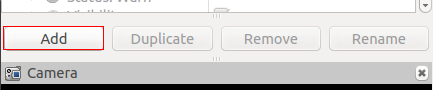
\includegraphics[scale=0.5]{Add.png} 
  \caption{Bouton Add}
\end{figure}
Il faut également enregistrer sa configuration en faisant un \upshape \emph{Ctrl+S}.


\newpage
\section{Navigation}
\label{sec:Navigation}


Nous avons remarqué lors de nos expérimentations sur les TurtleBot qu'un des TurtleBot (le TurtleBot 3) avait des roues folles légèrement plus petites que celles des autres robots. Cette différence permet au robot d'éviter de frotter au sol lors de ces mouvements rotatifs, et lui permet de se déplacer de manière beaucoup plus fluide et plus stable. Pour les tests qualitatifs et les démonstrations, il sera donc plus intéressant d'utiliser ce TurtleBot, ou au moins de démonter ses roues et de les intégrer sur le TurtleBot utilisé.\\

De plus, les conditions d'illumination de l'environnement peuvent gêner la navigation du TurtleBot. En effet, une lumière trop importante peut entraîner une mauvaise visualisation voire une incapacité à visualiser les AR Codes par la Kinect. \\

Tout d'abord, allumez le TurtleBot (il y a un bouton sur le côté de la base du robot). Ensuite, allumez le PC TurtleBot. Nous allons maintenant lancer tous les noeuds ROS dont notre application aura besoin pour fonctionner.

\subsection{Sur le PC TurtleBot}

Il faut d'abord télécharger tout le code source de notre projet sur le PC Turtlebot (voir section 1.3.2).

\subsubsection{Fonctionnalités basiques}
\label{sec:navigation2}

Si vous utilisez le PC TurtleBot, ouvrez trois terminaux et exécutez chacune des commandes suivantes sur un terminal différent, pour activer les fonctionnalités minimales et de vision, et pour lancer le filtre de Kalman :

\begin{itemize}
\item[]  \begin{verbatim}> roslaunch turtlebot_bringup minimal.launch \end{verbatim}
\item[]  \begin{verbatim}> roslaunch turtlebot_visual_navigation alvar.launch \end{verbatim}
\item[]  \begin{verbatim}> roslaunch turtlebot_visual_navigation Kalman.launch \end{verbatim}
\end{itemize}

\subsubsection{Navigation}
\label{sec:navigation}

Pour lancer notre programme, il faut tout d'abord lancer RViz, puis lancer l'exécutable de notre code :

\begin{itemize}
\item[] \begin{verbatim}> roslaunch turtlebot_visual_navigation navigation.launch \end{verbatim}
\item[]  \begin{verbatim}> rosrun turtlebot_visual_navigation Navigation \end{verbatim}
\end{itemize}

Vous pouvez maintenant voir l'interface de RViz, le TurtleBot ainsi que tous les markers.
Pour faire se déplacer le TurtleBot, il suffit de créer un 2D Nav Goal en cliquant sur le bouton du même nom. On positionne ensuite le NavGoal directement sur la carte.\\
\begin{figure}[!h]
  \centering
  \noindent
\includegraphics[scale=0.5]{2DNavGoal.png} 
  \caption{Bouton 2D Nav Goal}
\end{figure}

\subsection{Depuis un PC externe}

Il est possible (et même conseillé dans le cadre de notre projet) de lancer l'application depuis un autre PC que celui de la TurtleBot.
Il est tout de même préférable de lancer les fichiers \upshape \emph{minimal.launch}, \upshape \emph{alvar.launch} et \upshape \emph{Kalman.launch} depuis le PC TurtleBot (voir section \ref{sec:navigation2}).

\subsubsection{Fonctionnalités de base}

Il est tout de même possible de lancer les fichiers \upshape \emph{minimal.launch}, \upshape \emph{alvar.launch} et \upshape \emph{Kalman.launch} depuis un PC externe. Il faut pour cela se connecter au PC TurtleBot en premier lieu.
Dans un premier terminal, exécutez les commandes suivantes :

\begin{itemize}
\item[]  \begin{verbatim}> ssh turtlebot@<TURTLEBOTP_IP> \end{verbatim}
\item[]  \begin{verbatim}> roslaunch turtlebot_bringup minimal.launch \end{verbatim}
\end{itemize}

Dans un second terminal, exécutez les commandes suivantes :

\begin{itemize}
\item[]  \begin{verbatim}> ssh turtlebot@<TURTLEBOTP_IP> \end{verbatim}
\item[]  \begin{verbatim}> roslaunch turtlebot_visual_navigation alvar.launch \end{verbatim}
\end{itemize}

Dans un troisième terminal, exécutez les commandes suivantes :

\begin{itemize}
\item[]  \begin{verbatim}> ssh turtlebot@<TURTLEBOTP_IP> \end{verbatim}
\item[]  \begin{verbatim}> roslaunch turtlebot_visual_navigation Kalman.launch \end{verbatim}
\end{itemize}

\subsubsection{Navigation}

Pour lancer notre application depuis un PC externe, on lance d'abord RViz avec la commande :
\begin{itemize}
\item[]  \begin{verbatim}> roslaunch turtlebot_visual_navigation navigation.launch \end{verbatim}
\end{itemize}

Puis on lance l'application avec :
\begin{itemize}
\item[]  \begin{verbatim}> rosrun turtlebot_visual_navigation Navigation \end{verbatim}
\end{itemize}

\begin{comment}

On se connecte ensuite au PC Turtlebot et on lance notre programme grâce aux commandes suivantes :

\begin{itemize}
\item[]  \begin{verbatim}> ssh -X turtlebot@<TURTLEBOTP_IP> \end{verbatim}
\item[]  \begin{verbatim}> rosrun turtlebot_visual_navigation Navigation \end{verbatim}
\end{itemize}

\end{comment}

Vous pouvez maintenant voir l'interface de RViz, le TurtleBot ainsi que tous les markers.
Pour faire se déplacer le TurtleBot, il suffit de créer un 2D Nav Goal en cliquant sur le bouton du même nom. On positionne ensuite le NavGoal directement sur la carte.\\
\begin{figure}[!h]
  \centering
  \noindent
\includegraphics[scale=0.5]{2DNavGoal.png} 
  \caption{Bouton 2D Nav Goal}
\end{figure}


\newpage
\section*{ANNEXE}

\section{Un exemple de lancement depuis le PC TurtleBot}

On exécute toutes les commandes depuis le PC TurtleBot.
Dans un premier temps, il faut être sûr que le programme compile. \\
Placez-vous dans le workspace et exécutez la commande :
\begin{itemize}
\item[] \begin{verbatim}> catkin_make \end{verbatim}
\end{itemize}

Une fois que le programme est compilé, on peut dans un premier terminal, lancer la commande :
\begin{itemize}
\item[] \begin{verbatim}> roslaunch turtlebot_bringup minimal.launch \end{verbatim}
\end{itemize}

Dans un second terminal, lancez la commande :
\begin{itemize}
\item[] \begin{verbatim}> roslaunch turtlebot_visual_navigation alvar.launch \end{verbatim}
\end{itemize}

Dans un troisième terminal, lancez la commande :
\begin{itemize}
\item[] \begin{verbatim}> roslaunch turtlebot_visual_navigation Kalman.launch \end{verbatim}
\end{itemize}

Dans un quatrième terminal, lancez la commande :
\begin{itemize}
\item[] \begin{verbatim}> roslaunch turtlebot_visual_navigation navigation.launch \end{verbatim}
\end{itemize}

Dans un cinquième terminal, lancez la commande :
\begin{itemize}
\item[] \begin{verbatim}> rosrun turtlebot_visual_navigation Navigation \end{verbatim}
\end{itemize}

\section{Un exemple de lancement depuis un PC externe}

On va exécuter trois commandes depuis le PC TurtleBot. Dans un premier terminal, lancez :
\begin{itemize}
\item[] \begin{verbatim}> roslaunch turtlebot_bringup minimal.launch \end{verbatim}
\end{itemize}

Dans un second terminal, lancez la commande :
\begin{itemize}
\item[] \begin{verbatim}> roslaunch turtlebot_visual_navigation alvar.launch \end{verbatim}
\end{itemize}

Dans un troisième terminal, lancez la commande :
\begin{itemize}
\item[] \begin{verbatim}> roslaunch turtlebot_visual_navigation Kalman.launch \end{verbatim}
\end{itemize}

\vspace{0.5cm}
Allez maintenant sur un PC autre que le PC TurtleBot. Dans un premier temps, il faut être sûr que le programme compile. \\
Placez-vous dans votre workspace et exécutez la commande :
\begin{itemize}
\item[] \begin{verbatim}> catkin_make \end{verbatim}
\end{itemize}

Une fois que le programme est compilé, on peut dans un premier terminal, lancer la commande :
\begin{itemize}
\item[] \begin{verbatim}> roslaunch turtlebot_visual_navigation navigation.launch \end{verbatim}
\end{itemize}

Dans un second terminal, lancez la commande :
\begin{itemize}
\item[] \begin{verbatim}> rosrun turtlebot_visual_navigation Navigation \end{verbatim}
\end{itemize}



\end{document}